% NEXT: 2.1 背景・2.2 目的 の第一稿（9/9）を読んで直す。次に書くのは 2.7.5 取得条件と 2.7.6 参照グリッド（論文 Methods を日本語に）〔初期値〕
% 第2章: QPI による長期1細胞計測系の構築
% 2026-09-08 に橋本幹弘さんの博論（48136）の形に組み替えた。
% 2026-09-09 に節を確定し、見出しを日本語にした。
%   背景 → 目的 → 原理 → 再構成 → 光学系 → デバイス → 細胞と計測 → 画像解析 → 性能評価 → 考察 → まとめ
%   本文は節の下に移しただけで書き直していない。英語と日本語が混ざったまま。
\chapter{QPIによる長期1細胞計測系の構築}

\section{背景}
\label{sec:background}
% 2026-09-09 に Claude が、論文 qpi-methods/sentence/10_intro.tex と plot/2_measurement_system.md の 2.1 から起こした第一稿。
% 橋本博論 48136 の 2.1（2.1.1 既存技術の問題点 → 2.1.2 必要条件 → 2.2 目的1文）の形に合わせた。本人が読んで直す。
% 屈折率増分は文献値として 0.18〜0.19 mL/g と書いた。解析で使う1つの値は 2.8.7 で決める（コードの値に合わせる）。

\subsection{細胞質の乾燥質量密度と既存の計測法}

細胞質の乾燥質量密度、すなわち細胞質の非水成分の濃度は、細胞内の拡散、反応速度、相分離に影響する\cite{ellis2001crowding,delarue2018mtorc1,molines2022cytoplasm}。集団の平均で見ると、密度は増殖速度が数倍変わっても一定に保たれる\cite{kubitschek1984independence,kubitschek1985buoyant}。一方、1細胞の水準では生合成と体積成長が脱共役しうる。G1 期に停止させた出芽酵母は大きく成長して細胞質が希釈され\cite{neurohr2019excessive}、分裂酵母では体積成長を一時的に止めると密度が上がる\cite{knapp2019decoupling}。通常の細胞周期の進行でも密度は変わる\cite{odermatt2021variations,zlotekzlotkiewicz2015optical}。それでも、同じ条件にある細胞どうしの密度の差は数\%にとどまる\cite{oldewurtel2021robust,odermatt2021variations,liu2022uniformity}。第3章で扱うグルコース飢餓下の密度変化を1細胞で捉えるには、この数\%の差を分解する精度で、同じ細胞を数日にわたって測り続ける計測が要る。

屈折率は分子濃度の指標である。溶液の屈折率 $n$ は溶質の質量濃度 $C$ に対して $n = n_0 + \alpha C$ と線形に増える。比例係数 $\alpha$（屈折率増分）はタンパク質と核酸でほぼ共通の値 $0.18$〜$0.19~\mathrm{mL/g}$ をとり、細胞内の濃度範囲で線形性が保たれる\cite{barer1952interference,barer1954refractive,zhao2011distribution,zangle2014live}。したがって、細胞と培地の屈折率差を測れば、細胞質の乾燥質量濃度が求まる。

1細胞の密度を測る方法には次のものがある。浮遊密度は Percoll などの密度勾配遠心で測る\cite{woldringh1981variation,kubitschek1985buoyant,bryan2010measurement}。集団を分画する測定なので同じ細胞の時系列は得られず、遠心と勾配媒体が細胞の環境を変える。懸濁マイクロチャネル共振器（SMR）は1細胞の浮遊質量を高い精度で測り、密度の異なる2種類の液中での測定から密度を求める\cite{grover2011measuring,bryan2010measurement}。細胞を流路に流して測るので、同じ細胞を数日追うことには向かない。蛍光排除法は体積を測る方法で、質量の測定と組み合わせて密度を出す\cite{zlotekzlotkiewicz2015optical}が、培地に蛍光色素を加える必要がある。ラマン散乱を用いる方法は分子種ごとの濃度を無標識で与える\cite{oh2022protein}が、装置と取得時間の点で、多数の視野を数分間隔で数日撮る用途には向かない。

定量位相イメージング（QPI）は、細胞を透過した光の位相遅れ $\Delta\phi = (2\pi/\lambda)\int (n_{\mathrm{cell}} - n_0)\,dz$ を定量する\cite{barer1952interference,popescu2006diffraction,park2018quantitative,nguyen2022quantitative}。位相の面積分は乾燥質量に比例し、体積と合わせれば密度になる。標識も固定も要らず、1枚の露光で1視野の位相像が得られるので、長期のタイムラプスに使える。分裂酵母でも、細胞周期内の密度変動が QPI で測られている\cite{rappaz2009noninvasive,odermatt2021variations}。ただし、系譜に沿って密度を追った記録は1〜数周期にとどまり\cite{odermatt2021variations,liu2020computationally}、世代をまたいだ細胞間のばらつきがどう振る舞うかは分かっていない。

\subsection{長期1細胞密度計測系の必要条件}
\label{sec:requirements}

前項の方法を、分裂酵母1細胞の密度を飢餓下で数日にわたって追うという目的に照らすと、計測系に必要な条件は次の4つになる。

\begin{enumerate}
\item 長期の1細胞追跡。同じ細胞を同じ視野に数日とどめ、指数関数的に増える子孫を系外に除き、培地を一定に保つか任意の時刻に交換できること。細胞を行き止まりの細い流路に1列で閉じ込め、主流路で培地を流す mother machine がこれを満たす\cite{wang2010robust,nakaoka2017aging}。
\item 無標識・非侵襲で、1枚の露光から位相像が得られること。多数の視野を数分間隔で数日撮るので、機械的な走査や複数枚の取得を要する方式は取得時間と安定性の点で不利である。数日の記録では振動と光学系のずれが避けられないので、物体光と参照光が同じ光路を通る common-path 型の干渉計が要る。
\item 位相ノイズが、測りたい密度差に対応する位相差より十分小さいこと。同一条件での細胞間の密度差は数\%なので、位相像のノイズはその位相差の数分の一以下でなければならない。
\item 背景の位相を細胞の無い領域から取れること。QPI では照明光の位相分布を試料の無い領域で測って差し引くが、mother machine の観察チャネルは細胞で埋まり、細胞のそばに培地だけの領域が残らない。背景をどこから取るかを別に決める必要がある。
\end{enumerate}

このほか、数千フレームの位相像から細胞の輪郭、系譜、体積を自動で取り出す解析が要る。第1・第2の条件は既存の要素（mother machine と common-path off-axis 干渉計）の組み合わせで満たせる。第3の条件は光学系の設計（\ref{sec:optics} 節）と性能評価（\ref{sec:performance} 節）で示す。第4の条件は既存の方法では満たされないので、本研究では計測前にステージ変位のグリッドで参照像を記録する方式を導入した（\ref{sec:grid_acq} 節、\ref{sec:bgsub} 節）。

% 旧: なんで他の密度測定方法ではなく、QPIを用いたのかまで書きたかったら、generalな測定方法を挙げていって、この方法が良かったみたいなことを書けばよくて、その際には
% 旧: \cite{nguyen2022quantitative}
% 旧: non invasive way of 
%
%
%
% 旧: It has been found that, for most biological molecules, including proteins and nucleic acids, the values of γ are close to 0.19 mL/g (\href{https://www.sciencedirect.com/science/chapter/bookseries/pii/S1063582318300024\#bib244}{Theisen, Johann, Deacon, \& Harding, 2000}), and the linearity is maintained for a wide range of concentrations \cite{zangle2014live}
% 旧: (\href{https://www.sciencedirect.com/science/chapter/bookseries/pii/S1063582318300024\#bib12}{Barer and Tkaczyk, 1954}, \href{https://www.sciencedirect.com/science/chapter/bookseries/pii/S1063582318300024\#bib278}{Zangle and Teitell, 2014}, \href{https://www.sciencedirect.com/science/chapter/bookseries/pii/S1063582318300024\#bib282}{Zhao et al., 2011}). Therefore, refractive index measurement is a rather direct approach to determination of concentration of molecules in cell.

\section{目的}
\label{sec:aim}
分裂酵母を対象に、\ref{sec:requirements} 節の4条件を満たす、QPI による長期1細胞乾燥質量密度計測系を構築する。common-path off-axis ディジタルホログラフィの光学系、mother machine、ステージ変位のグリッドによる参照像の取得、位相像から乾燥質量密度までの解析パイプラインを一体として作り、その性能を位相ノイズ、参照像の登録精度、ドリフト、既知シフトの回収、濃度校正の直線性で評価する（\ref{sec:performance} 節）。この計測系を第3章のグルコース飢餓実験に用いる。

\section{定量位相イメージングの原理}
% TODO: ここの導出は AppendixA と重なっている。本文には結果に必要な分だけ残し、
% 導出は AppendixA へ落とすかどうかを決める（2026-09-09 の枠で判断）。
Differences in refractive index between a cell and its environment are imprinted upon light as different delays to the phase of light oscillations. Because frequencies of visible light are very high (400–800 THz), its oscillations cannot be directly recorded by imaging sensors. To become detectable, phase delay must be converted into measurable intensity. This is done in standard phase contrast and differential interference contrast microscopes. Quantification of the phase is accomplished by a group of methods known as quantitative phase imaging (QPI)
QPI is based on transmitted illumination that crosses a refractive sample (Fig. 1). When the cell's refractive index varies both across the sample and in depth, the relative phase accrued by light passing through the cell at horizontal position x is
\begin{equation}
    \Delta \phi(x)= \frac{2\pi}{\lambda} \int_0^{h(x)}[n_{cell}(x,z) - n_0]dz
\end{equation}
where $z$ denotes depth within the sample, $h(x)$ is the cell thickness profile, $n_{\text{cell}}$ is the cell's refractive index (which may vary depending on the position), $n_0$ is a constant refractive index of the medium, and $\lambda$ is the wavelength of light. Scattering is assumed insignificant in this model. 
\begin{figure}
    \centering
    \includegraphics[width=0.5\linewidth]{example-image}
    \caption{A diagram showing accumulation of phase delay of light passing through a cell}
    \label{fig:phase_delay}
\end{figure}
\subsection{共通光路法}
common path QPI methods implement a considerably more compact interferometer after the sample. In this geometry, the two interfering light beams propagate through many of the same optical components, increasing robustness to vibrations and misalignments of the system as well as generally reducing the system's footprint. Because they can be placed after the sample, common-path systems can also be easily implemented at the output port of a microscope.
だから長期のタイムラプスに最適。

\subsection{光の伝搬と角スペクトル法}
The propagation of monochromatic light in a homogeneous medium is governed by the Helmholtz equation:
\begin{equation}
\nabla^2 U(\mathbf{r}) + k^2 U(\mathbf{r}) = 0,
\end{equation}
where $k = 2\pi n/\lambda$ is the wavenumber, $n$ is the refractive index, $\lambda$ is the wavelength, and $\nabla^2 = \partial^2/\partial x^2 + \partial^2/\partial y^2 + \partial^2/\partial z^2$ is the Laplacian operator. The solution can be expressed as a superposition of plane waves with different spatial frequencies $(f_x, f_y)$:
\begin{equation}
U(x,y,z) = \int\int \tilde{U}(f_x, f_y, z) e^{2\pi i(f_x x + f_y y)} df_x df_y,
\end{equation}
where $\tilde{U}(f_x, f_y, z)$ is the angular spectrum. Substituting this into the Helmholtz equation yields the dispersion relation:
\begin{equation}
k_x^2 + k_y^2 + k_z^2 = k^2,
\end{equation}
where $k_x = 2\pi f_x$, $k_y = 2\pi f_y$, and
\begin{equation}
k_z = \sqrt{k^2 - k_x^2 - k_y^2} = \sqrt{k^2 - (2\pi f_x)^2 - (2\pi f_y)^2}
\end{equation}
is the z-component of the wavevector.

For propagation from $z=0$ to $z=d$, each plane wave component acquires a phase factor $e^{i k_z d}$:
\begin{equation}
\tilde{U}(f_x, f_y, d) = \tilde{U}(f_x, f_y, 0) \cdot e^{i k_z d}.
\end{equation}
The field at distance $d$ is then obtained by inverse Fourier transformation:
\begin{equation}
U(x,y,d) = \mathcal{F}^{-1}\left\{\tilde{U}(f_x, f_y, 0) \cdot e^{i k_z d}\right\}.
\end{equation}

\subsection{対物レンズによる帯域制限}
\label{sec:bandlimit}

An objective lens with numerical aperture NA acts as a spatial frequency filter, passing only components with $\sqrt{f_x^2 + f_y^2} \leq \mathrm{NA}/\lambda$. The transmitted field spectrum is
\begin{equation}
\tilde{U}_{\mathrm{transmitted}}(f_x, f_y) = \tilde{U}_0(f_x, f_y) \cdot P(f_x, f_y),
\end{equation}
where $P(f_x, f_y)$ is the pupil function:
\begin{equation}
P(f_x, f_y) = \begin{cases}
1 & \text{if } \sqrt{f_x^2 + f_y^2} \leq f_{\mathrm{cutoff}} = \mathrm{NA}/\lambda \\
0 & \text{otherwise}
\end{cases}.
\end{equation}
This band-pass limitation determines the spatial resolution through the Abbe diffraction limit:
\begin{equation}
\label{eq:abbe}
\Delta x_{\mathrm{Abbe}} = \frac{\lambda}{\mathrm{NA}}
\end{equation}
for coherent illumination.

\subsection{4f光学系における光の伝搬}

A 4f optical system consists of two lenses with focal length $f$ arranged such that the object plane, Fourier plane, and image plane are separated by distances $f$. This configuration performs spatial Fourier transformation and imaging, and is widely used in spatial light modulation, optical filtering, and holographic imaging systems \cite{goodman2005}.

\subsubsection{系の構成}

The 4f system comprises the following elements (Fig.~\ref{fig:4f_system}):
\begin{itemize}
\item Object plane at $z = 0$
\item First lens (L1) with focal length $f$ at $z = f$
\item Fourier plane at $z = 2f$
\item Second lens (L2) with focal length $f$ at $z = 3f$
\item Image plane at $z = 4f$
\end{itemize}

\subsubsection{単レンズによるFourier変換}

When an object is placed at the front focal plane of a lens with focal length $f$, the field at the back focal plane (Fourier plane) is proportional to the spatial Fourier transform of the object field \cite{goodman2005}:
\begin{equation}
U_F(x_F, y_F) = \frac{e^{ikf}}{i\lambda f} e^{i\frac{k}{2f}(x_F^2 + y_F^2)} \mathcal{F}\{U_0(x_0, y_0)\}\bigg|_{f_x = \frac{x_F}{\lambda f}, f_y = \frac{y_F}{\lambda f}}
\end{equation}
where $U_0$ is the object field, and the quadratic phase factor $\exp[ik(x_F^2 + y_F^2)/(2f)]$ represents the spherical wavefront curvature at the Fourier plane.

The spatial frequency components $(f_x, f_y)$ are mapped to coordinates in the Fourier plane according to:
\begin{equation}
f_x = \frac{x_F}{\lambda f}, \quad f_y = \frac{y_F}{\lambda f}
\end{equation}

\subsubsection{4f系における空間フィルタリング}

A spatial filter (e.g., pinhole, amplitude mask) placed at the Fourier plane modifies the spatial frequency spectrum. The filter function $P(x_F, y_F)$ multiplies the Fourier-domain field:
\begin{equation}
U_F^+(x_F, y_F) = U_F(x_F, y_F) \cdot P(x_F, y_F)
\end{equation}

The second lens performs an inverse Fourier transformation, yielding the filtered image at $z = 4f$. For a symmetric 4f system without filtering ($P = 1$), the output is an inverted image of the input:
\begin{equation}
U_i(x_i, y_i) = -U_0(-x_i, -y_i) \cdot e^{i4kf}
\end{equation}
where the negative sign indicates spatial inversion in both transverse directions.

\subsection{干渉による位相の回復}

Since image sensors can only measure intensity $I = |U|^2$, the phase information $\phi$ in the complex field $U = A e^{i\phi}$ is lost upon detection. To recover the phase, we interfere the object field $U_s = A_s e^{i\phi_s}$ with a known reference field $U_r = A_r e^{i\phi_r}$. The detected intensity is
\begin{equation}
\label{eq:interference}
I = |U_s + U_r|^2 = |U_s|^2 + |U_r|^2 + U_s \cdot U_r^* + U_s^* \cdot U_r,
\end{equation}
which can be expanded as
\begin{equation}
I = A_s^2 + A_r^2 + 2A_s A_r \cos(\phi_s - \phi_r).
\end{equation}
The phase difference $\phi_s - \phi_r$ modulates the intensity as interference fringes. However, in an on-axis configuration, all four terms in \eqref{eq:interference} occupy the same region in Fourier space, preventing isolation of the phase-containing term $U_s \cdot U_r^*$.

\subsection{off-axis配置}

To separate the interferometric components in Fourier space, we introduce a carrier frequency by giving the object field an off-axis wavevector $(k_m^{\mathrm{off-axis}}, k_n^{\mathrm{off-axis}})$, where $(m, n)$ denote discrete pixel indices. In our common-path system, the reference field is spatially filtered by a pinhole at the Fourier plane to produce a quasi-plane wave:
\begin{equation}
U_r = A_r,
\end{equation}
while the object field carries the off-axis wavevector introduced by the Ronchi ruling grating:
\begin{equation}
U_s = A_s e^{i\phi_s} e^{-i(k_m^{\mathrm{off-axis}} m + k_n^{\mathrm{off-axis}} n)}.
\end{equation}
The interference pattern then becomes
\begin{equation}
I_{m,n} = |U_s|^2 + |U_r|^2 + U_s \cdot U_r^* + U_s^* \cdot U_r = A_s^2 + A_r^2 + 2A_r A_s \cos[\phi_s - k_m^{\mathrm{off-axis}} m - k_n^{\mathrm{off-axis}} n].
\end{equation}

Taking the 2D Fourier transform with reciprocal coordinates $(p,q)$, we obtain
\begin{equation}
\tilde{I}(p,q) = \tilde{I}_{\mathrm{DC}}(p,q) + \mathcal{F}\{U_s \cdot U_r^*\}(p + k_m^{\mathrm{off-axis}}, q + k_n^{\mathrm{off-axis}}) + \mathcal{F}\{U_s^* \cdot U_r\}(p - k_m^{\mathrm{off-axis}}, q - k_n^{\mathrm{off-axis}}).
\end{equation}
The three components are now spatially separated in Fourier space. By selecting the +1st-order sideband and applying inverse Fourier transformation, the complex field $U_s$ is isolated and its phase $\phi_s = \arg(U_s)$ is extracted.

\subsection{off-axisホログラムの形成}

In off-axis DH, the interference patterns between the object field and reference field are captured with an image sensor. Assuming $z = 0$ as the sample location, the object field at the sensor is
\begin{equation}
U_{s,m,n} = \frac{1}{M^2} A_s \exp[i\phi_{m,n}] \exp[-i(k_m^{\mathrm{off-axis}} m + k_n^{\mathrm{off-axis}} n)],
\end{equation}
where $M$ is the magnification, $A_s$ is the object-field amplitude, $(k_m^{\mathrm{off-axis}}, k_n^{\mathrm{off-axis}})$ is the off-axis carrier frequency introduced by the Ronchi ruling grating, and $\phi_{m,n}$ contains the optical phase delay induced by the sample. The reference field is
\begin{equation}
U_{r,m,n} = A_r,
\end{equation}
which is approximately constant across the field of view after spatial filtering by the pinhole at the Fourier plane.

The recorded hologram intensity at pixel $(m,n)$ is
\begin{equation}
I_{m,n}^{\mathrm{DH}} = \left|U_{s,m,n} + U_{r,m,n}\right|^2 = |U_{s,m,n}|^2 + |U_{r,m,n}|^2 + U_{s,m,n} \cdot U_{r,m,n}^* + \mathrm{c.c.}
\end{equation}
This can be separated into interferometric terms ($J_{m,n}^{\mathrm{int}} e^{-i(k_m^{\mathrm{off-axis}}m + k_n^{\mathrm{off-axis}}n)}$ and its complex conjugate) and noninterferometric term ($J_{m,n}^{\mathrm{non-int}}$) as
\begin{equation}
\label{eq:hologram_DH}
I_{m,n}^{\mathrm{DH}} = J_{m,n}^{\mathrm{non-int}} + J_{m,n}^{\mathrm{int}} e^{-i(k_m^{\mathrm{off-axis}}m + k_n^{\mathrm{off-axis}}n)} + (J_{m,n}^{\mathrm{int}})^* e^{+i(k_m^{\mathrm{off-axis}}m + k_n^{\mathrm{off-axis}}n)},
\end{equation}
where $J_{m,n}^{\mathrm{non-int}} = |U_{s,m,n}|^2 + |U_{r,m,n}|^2$ and $J_{m,n}^{\mathrm{int}} = U_{s,m,n} \cdot U_{r,m,n}^*$.

\section{位相像の再構成}
\label{sec:reconstruction}
% 2026-09-09 に plot/2 の 2.4（P1〜P5）と paragraph/2 の T/E/I/B から日本語で書いた。英語の旧本文は git の ebf768f 以前にある。
% 図は figure-hub fig_qpi_reconstruction_overview v003（figure/qpi_fig_01_panel.pdf）。論文 Figure 1C（8/10 確定）に差し替えるなら figure-hub から取る。
% 円窓の半径は旧本文の (2πNA/λ)·N·Δp から 2π を外した。D_ap = 2⌊(NA/λ)·FOV⌋+1 = 511 と整合するのはこちら。

ホログラム1枚から位相像を得る手順は5段階である（図~\ref{fig:reconstruction}）\cite{takeda1982fourier}。第1に、ホログラム $I^{\mathrm{DH}}_{m,n}$ を2次元離散 Fourier 変換する。式~\eqref{eq:hologram_DH} より、そのスペクトルは
\begin{equation}
i_{p,q}^{\mathrm{DH}} = j_{p,q}^{\mathrm{non-int}} + j_{p+k_m^{\mathrm{off-axis}},\, q+k_n^{\mathrm{off-axis}}}^{\mathrm{int}} + j_{p-k_m^{\mathrm{off-axis}},\, q-k_n^{\mathrm{off-axis}}}^{\mathrm{int}*}
\end{equation}
の3成分からなる。$(p,q)$ は $(m,n)$ に共役な座標である。干渉項は off-axis の波数の分だけ原点から離れているので、3成分は Fourier 空間で分離している。第2に、$+1$ 次のサイドバンドの中心 $(p_{\mathrm{off}}, q_{\mathrm{off}})$ を求め、ホログラムに位相因子を掛けてサイドバンドを原点へ移す:
\begin{equation}
I_{m,n}^{(c)} = I_{m,n}^{\mathrm{DH}} \cdot e^{+i(k_m^{\mathrm{off-axis}}m + k_n^{\mathrm{off-axis}}n)}.
\end{equation}
第3に、原点を中心とする半径
\begin{equation}
r_{\mathrm{aperture}} = \frac{\mathrm{NA}}{\lambda} \cdot N \cdot \Delta p
\end{equation}
の円窓 $H_{p,q}$ で干渉項だけを切り出す。半径は離散 Fourier 座標の画素単位で、$N$ はホログラムの一辺の画素数、$\Delta p$ は物体面での画素ピッチである。この半径は、対物レンズの NA で決まる空間周波数のカットオフ（\ref{sec:bandlimit} 節）に対応する。第4に、切り出した成分を2次元逆 Fourier 変換して複素場を得て、その偏角を位相とする:
\begin{equation}
\phi_{m,n}^{\mathrm{meas}} = \arg[\mathrm{LP}(I_{m,n}^{(c)})].
\end{equation}
第5に、$\arg$ は $(-\pi, \pi]$ に折り返されているので、画素を信頼度の順に並べて $2\pi$ の飛びをつなぐ方法\cite{herraez2002fast}で unwrap する。円窓の半径は対物レンズの NA で決まるので、位相像の分解能は光学系で決まり、この処理で変わることはない。

この位相には、細胞による位相遅れのほかに、照明光の波面と流路の位相が乗っている。これを除くために、同じ視野で細胞の無い状態を撮った位相像（参照像）を引く。複素場の比の偏角をとれば位相の差になる:
\begin{equation}
\phi_{m,n} = \arg\left[\frac{\mathrm{LP}(I_{m,n}^{\mathrm{sample}} \cdot e^{+i(k_m^{\mathrm{off-axis}}m + k_n^{\mathrm{off-axis}}n)})}{\mathrm{LP}(I_{m,n}^{\mathrm{ref}} \cdot e^{+i(k_m^{\mathrm{off-axis}}m + k_n^{\mathrm{off-axis}}n)})}\right].
\end{equation}
照明光の波面と流路の位相は試料の像と参照像に共通なので、この差で消える。残るオフセットは細胞の無い領域の平均で除く。位相を光路長差に直すなら $\mathrm{OPD} = \phi\lambda/2\pi$ であるが、以降では位相 $\phi$（rad）のまま扱う。mother machine では細胞のそばに培地だけの領域が残らないので、参照像をどう取るかが問題になる。参照像の取得は \ref{sec:grid_acq} 節で、各フレームにどの参照像を対応させるかは \ref{sec:bgsub} 節で述べる。
\begin{figure}[H]
    \centering
    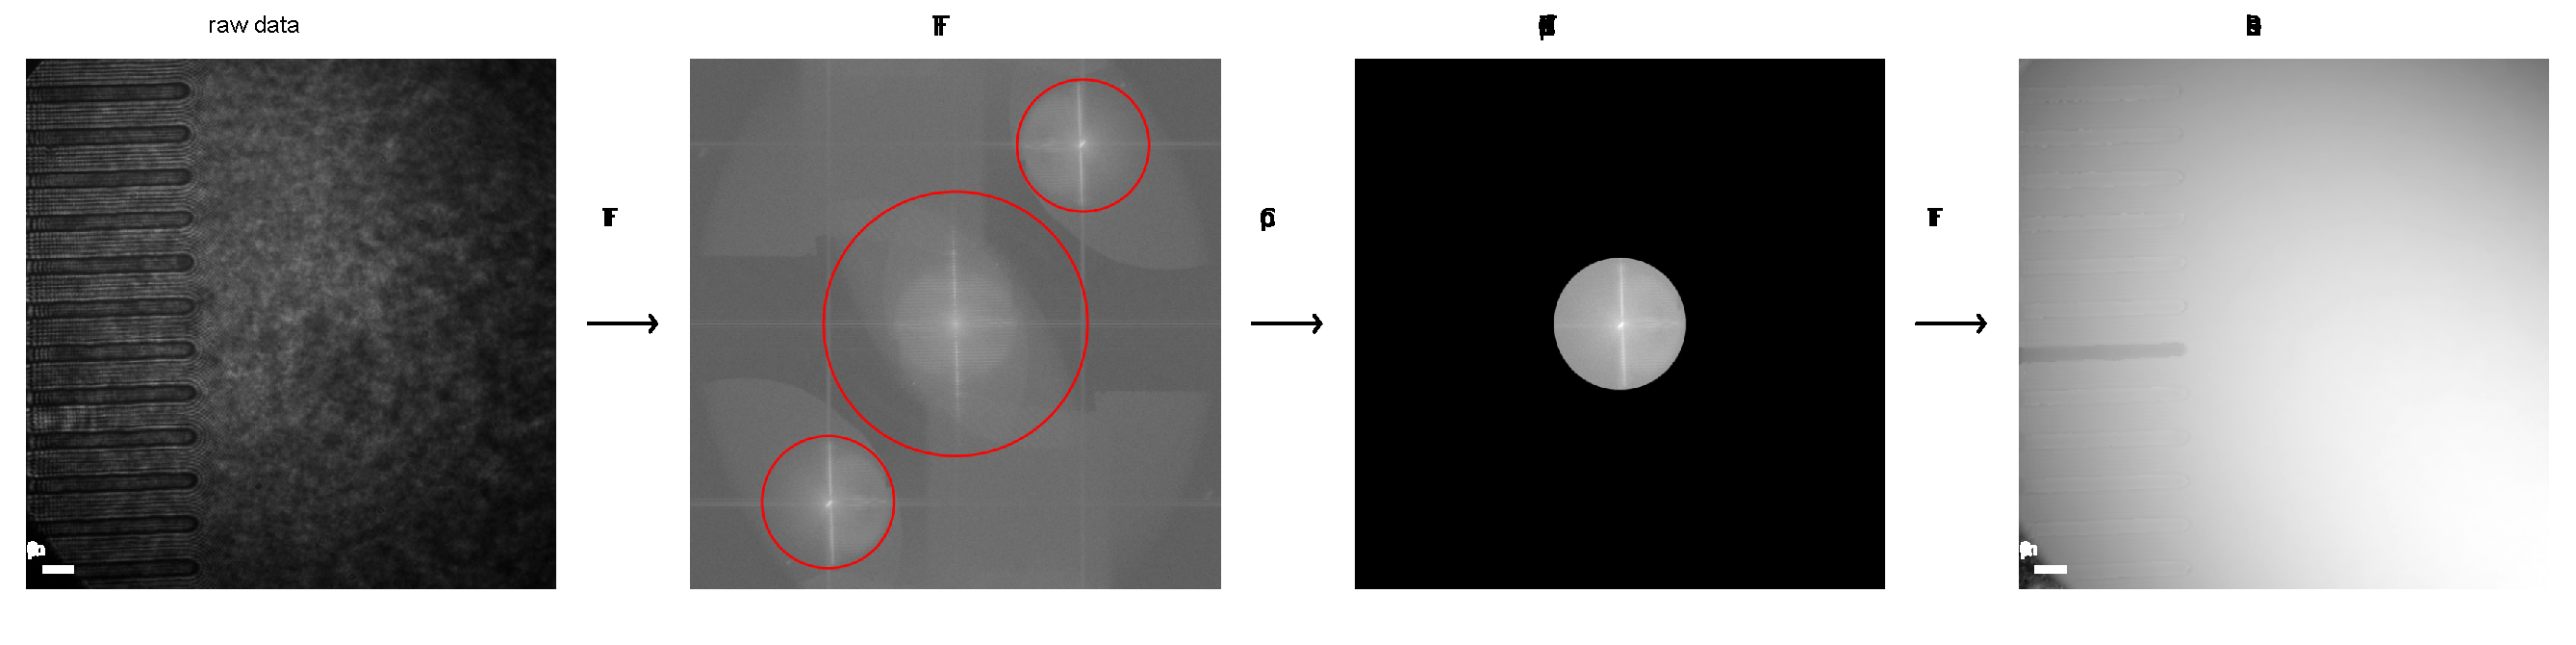
\includegraphics[width=0.95\linewidth]{figure/qpi_fig_01_panel.pdf}
    \caption{ホログラムから位相像までの再構成。左から、生のホログラム、その Fourier スペクトル、$+1$ 次サイドバンドを円窓で切り出したもの、逆 Fourier 変換して得た位相像。}
    \label{fig:reconstruction}
\end{figure}

\subsection{空間分解能とFourier面のパラメータ}

位相像の画素数と画素サイズは、対物レンズの NA と視野で決まる。コヒーレント照明での空間周波数のカットオフは
\begin{equation}
f_{\mathrm{cutoff}} = \frac{\mathrm{NA}}{\lambda}
\end{equation}
で、Abbe の分解限界（式~\eqref{eq:abbe}）に対応する。ホログラムが $N \times N$ 画素、物体面での画素ピッチが $\Delta p$ なら、視野は $\mathrm{FOV} = N \cdot \Delta p$ である。円窓の直径は画素単位で
\begin{equation}
D_{\mathrm{ap}} = 2 \,\mathrm{round}\!\left( \frac{\mathrm{NA}}{\lambda} \cdot \mathrm{FOV} \right) + 1
\end{equation}
となり（$\mathrm{round}$ は最も近い整数への丸め）、これがそのまま位相像の一辺の画素数になる。位相像の画素サイズは
\begin{equation}
\Delta p_{\mathrm{recon}} = \frac{\mathrm{FOV}}{D_{\mathrm{ap}}} \approx \frac{\lambda}{2\mathrm{NA}}
\end{equation}
で、分解能要素 $\lambda/\mathrm{NA}$ の半分である。すなわち位相像は、Nyquist の条件をちょうど満たす画素で組まれる。

サンプリングの条件は2段階ある。第1に、生のホログラムが折り返しを起こさないために
\begin{equation}
\Delta p < \frac{\lambda}{2 \cdot \mathrm{NA}}
\end{equation}
が要る。干渉縞を写すので、実際には 2--4 倍の余裕をとる。第2に、位相像では1分解能要素 $\lambda/\mathrm{NA}$ がおよそ2画素に対応する。生のホログラムの側の余裕は、干渉項が Nyquist を超えないという光学系の設計条件（\ref{sec:optics} 節の第2条件）と同じ要求である。

我々の系はこの条件を満たす。$\lambda = 658$ nm、NA $= 0.95$、倍率 $40\times$、カメラの画素 3.45 μm から、物体面の画素ピッチは $\Delta p = 3.45~\mu\mathrm{m}/40 = 86.25$ nm、視野は $2048 \times 86.25$ nm $= 176.64$ μm である。Abbe の分解限界は $658/0.95 = 692$ nm、Nyquist の条件は $\Delta p_{\mathrm{Nyquist}} = 658/(2 \times 0.95) = 346$ nm で、生のホログラムの余裕は $346/86.25 = 4.0$ 倍になる。円窓の直径は
\begin{equation}
D_{\mathrm{ap}} = 2 \,\mathrm{round}\!\left( \frac{0.95}{658 \times 10^{-9}} \times 176.64 \times 10^{-6} \right) + 1 = 2 \,\mathrm{round}(255.0) + 1 = 511
\end{equation}
画素で、位相像の画素サイズは $\Delta p_{\mathrm{recon}} = 176.64~\mu\mathrm{m}/511 = 346$ nm である。したがって位相像は $511 \times 511$ 画素、画素サイズ 0.346 μm となる。off-axis の波数 $k^{\mathrm{off-axis}}$ をどの範囲に置くかは、次節で光学系の設計条件として述べる。

\section{光学系}
\label{sec:optics}

\subsection{設計条件}

off-axis DH の光学系を設計するとき、満たすべき条件は2つある。第1に、off-axis の波数の大きさ $k^{\mathrm{off-axis}} = \sqrt{(k_m^{\mathrm{off-axis}})^2 + (k_n^{\mathrm{off-axis}})^2}$ が十分大きく、Fourier 空間で干渉項と非干渉項が重ならないことである。像面での干渉項の半径は $2\pi \mathrm{NA}/(\lambda M)$ で（$M$ は倍率）、非干渉項は周波数スペクトルの自己相関なので半径はその2倍の $2\pi \cdot 2\mathrm{NA}/(\lambda M)$ になる。したがって
\begin{equation}
k^{\mathrm{off-axis}} \geq 3 \left(\frac{2\pi \mathrm{NA}}{\lambda M}\right)
\label{eq:cond_overlap}
\end{equation}
が要る。第2に、干渉項の空間周波数が、センサの画素ピッチで決まる Nyquist 周波数を超えないことである。波数の向きは任意なので最も厳しいのは対角方向で、
\begin{equation}
\frac{k^{\mathrm{off-axis}}}{\sqrt{2}} + \frac{2\pi \mathrm{NA}}{\lambda M} \leq \frac{2\pi f_{\mathrm{pitch}}}{2}
\label{eq:cond_nyquist}
\end{equation}
が要る。$f_{\mathrm{pitch}}$ はセンサの画素ピッチの逆数である。2つを合わせると
\begin{equation}
\frac{2\pi \cdot 3\mathrm{NA}}{\lambda M} \leq k^{\mathrm{off-axis}} \leq \sqrt{2}\pi \left(f_{\mathrm{pitch}} - \frac{2\mathrm{NA}}{\lambda M}\right)
\label{eq:cond_range}
\end{equation}
になる。我々の系は NA $= 0.95$、$M = 40$、$\lambda = 658$ nm、画素ピッチ 3.45 μm（$f_{\mathrm{pitch}} = 1/3.45~\mu\mathrm{m} = 2.90 \times 10^5~\mathrm{m}^{-1}$）なので、下限は $3 \times 2\pi \times 0.95/(658 \times 10^{-9} \times 40) = 6.80 \times 10^5$ rad/m、上限は $\sqrt{2}\pi \left(2.90 \times 10^5 - 2 \times 0.95/(658 \times 10^{-9} \times 40)\right) = 9.68 \times 10^5$ rad/m である。この範囲は NA、倍率、画素ピッチだけで決まる。

\subsection{構成}

光学系を図~\ref{fig:qpi_optical_system}に示す。方式は回折位相顕微鏡（diffraction phase microscopy）、すなわち common-path off-axis DH である\cite{popescu2006diffraction}。光源は波長 658 nm、出力 20 mW のシングルモードファイバ出力の半導体レーザー（LP660-SF20, Thorlabs）で、ファイバコリメータ（CFC2-B, $f = 2.0$ mm, Thorlabs）で平行光にして試料を照明する。試料を透過した光は、倒立顕微鏡（Ti-E, Nikon）の $40\times$、NA 0.95 の乾燥系対物レンズ（CFI Plan Apochromat Lambda D, MRD70470, Nikon）で拡大され、顕微鏡の出力ポートに置いた像面で Ronchi 格子（120 lines/mm, \#66-342, Edmund Optics）により複数の回折次数に分けられる。各次数は像の空間情報をすべて持つ。焦点距離 200 mm のリレーレンズ2枚（ACT508-200-A, Thorlabs）で 4f 系を組み、その Fourier 面で 0 次光を直径 25 μm のピンホール（P25K, Thorlabs）で低域通過させて一様な参照光にし、1 次光はそのまま通して物体光にする。他の次数は遮る。2つの光は同じ光路を通り、センサ上で角度をもって干渉する。ホログラムは CMOS カメラ（acA2440-75um, Basler; $2448 \times 2048$ 画素、画素 3.45 μm、full-well 容量約 10 ke$^-$）で記録する。生のホログラムは $2048 \times 2048$ 画素を使い、再構成した位相像は \ref{sec:reconstruction} 節のとおり $511 \times 511$ 画素、画素 0.346 μm である。
\begin{figure}[H]
    \centering
    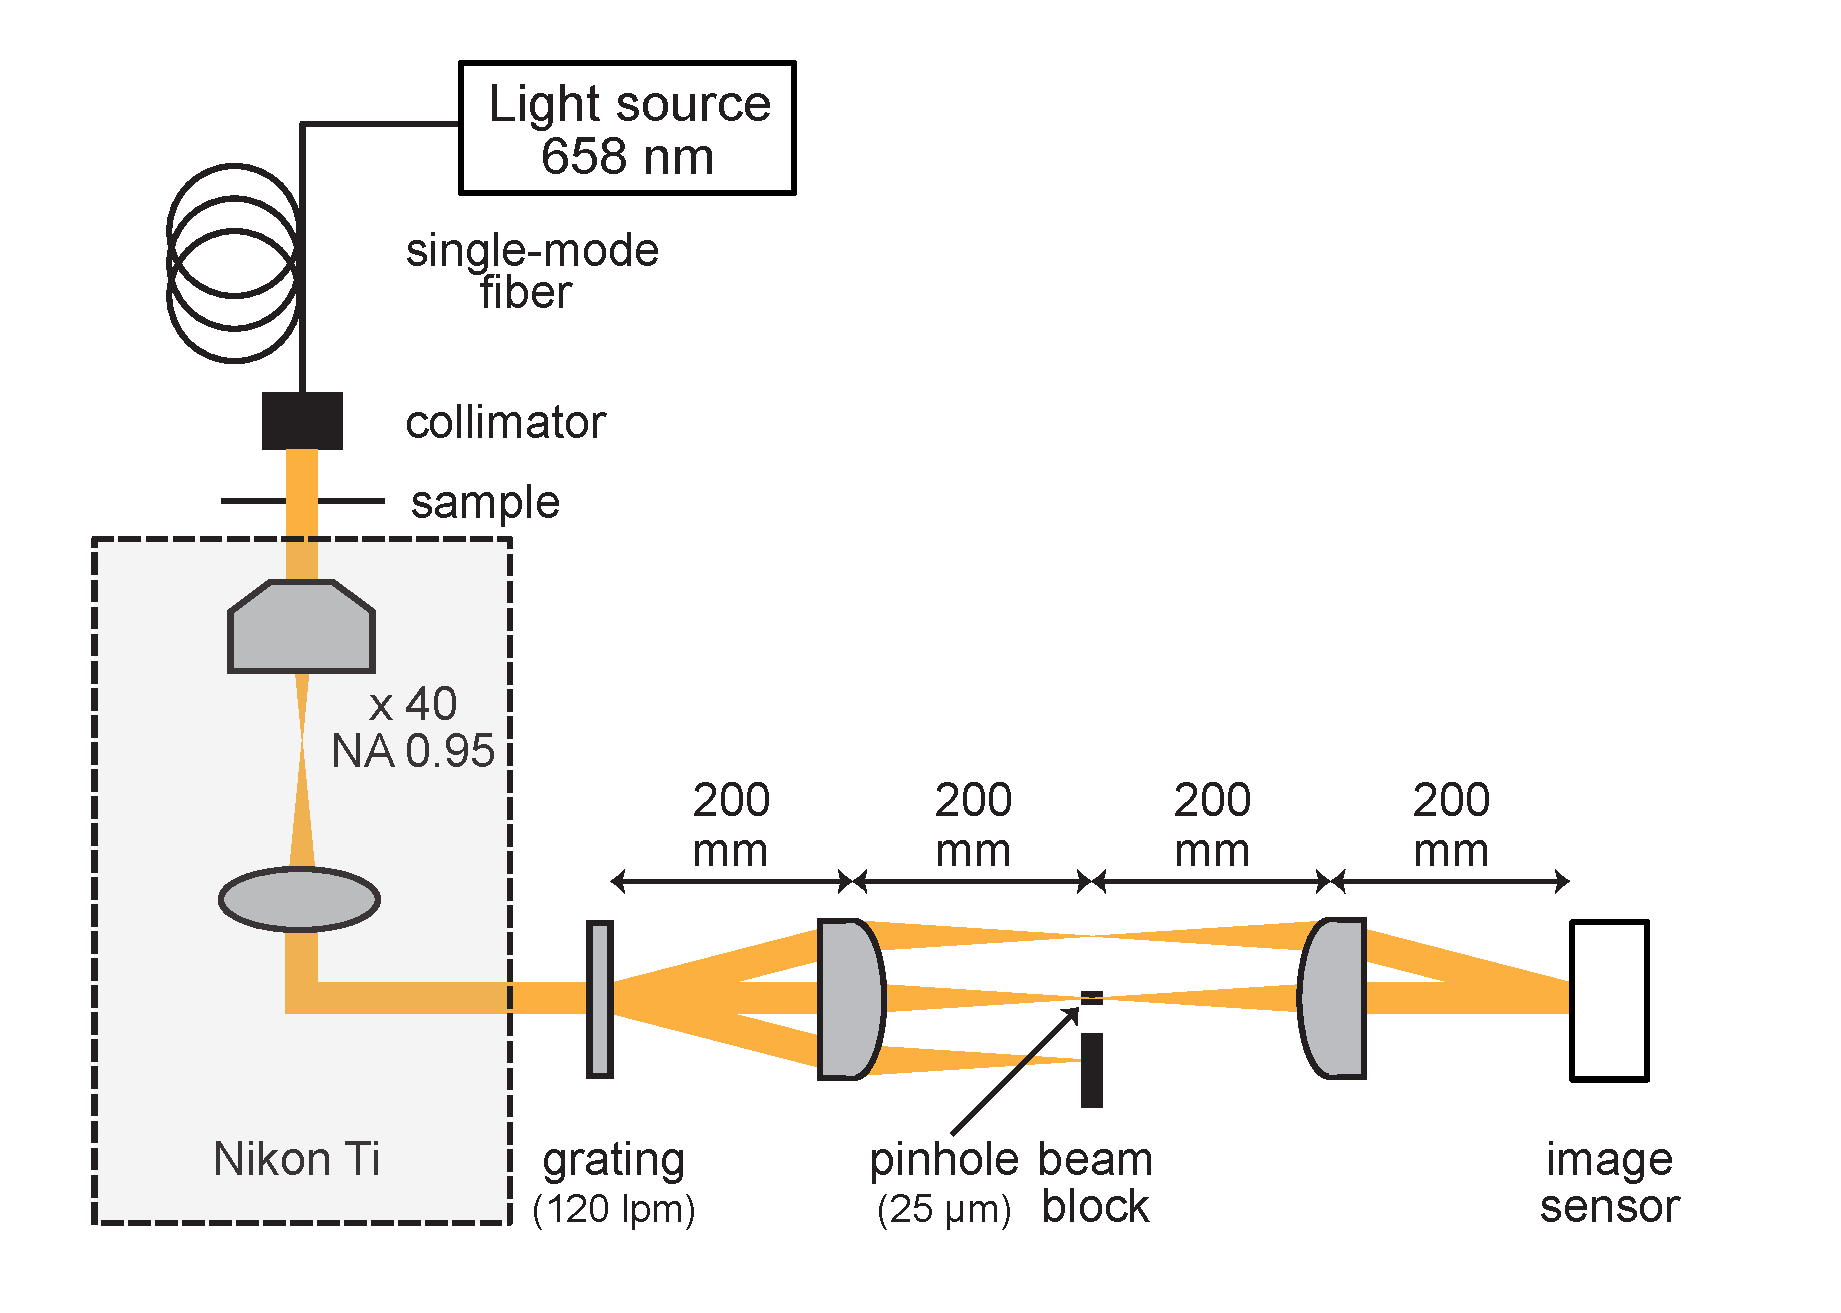
\includegraphics[width=0.85\linewidth]{figure/QPI optical systems.pdf}
    \caption{common-path off-axis ディジタルホログラフィの光学系。Ronchi 格子の $+1$ 次回折光を物体光、Fourier 面のピンホールで低域通過させた 0 次光を参照光にする。}
    \label{fig:qpi_optical_system}
\end{figure}

我々の系では、$k^{\mathrm{off-axis}}$ は試料と共役な像面に置いた格子の周期で決まる。4f リレーの倍率は 1 なので、センサ面での格子周期は 8.33 μm であり、
\begin{equation}
k^{\mathrm{off-axis}} = \frac{2\pi}{8.33~\mu\mathrm{m}} = 7.54 \times 10^5~\mathrm{rad/m}
\end{equation}
である。これは式~\eqref{eq:cond_range} の範囲 $6.80 \times 10^5 \leq k^{\mathrm{off-axis}} \leq 9.68 \times 10^5$ rad/m に入る。

\subsection{off-axis配置の検証}

設計どおりの off-axis 配置になっているかを、Fourier 空間でのキャリア周波数の実測で確かめた。$2048 \times 2048$ 画素のホログラムを Fourier 変換すると、直流成分は $(1024, 1024)$ に、$+1$ 次サイドバンドの中心は $(m_{\mathrm{off}}, n_{\mathrm{off}}) = (1623, 1621)$ にあった。中心からのずれは
\begin{equation}
\Delta m = 1623 - 1024 = 599, \quad \Delta n = 1621 - 1024 = 597
\end{equation}
画素で、その大きさは $\sqrt{599^2 + 597^2} = 845.8$ 画素である。センサ面での周波数分解能は
\begin{equation}
\Delta f_{\mathrm{sensor}} = \frac{1}{2048 \times 3.45~\mu\mathrm{m}} = \frac{1}{7.07~\mathrm{mm}} = 141.5~\mathrm{m}^{-1}
\end{equation}
なので、キャリアの空間周波数は $845.8 \times 141.5 = 1.20 \times 10^5$ cycles/m、波数にすると
\begin{equation}
k_{\mathrm{exp}}^{\mathrm{off-axis}} = 2\pi \times 1.20 \times 10^5 = 7.53 \times 10^5~\mathrm{rad/m}
\end{equation}
である。格子から計算した $7.54 \times 10^5$ rad/m と一致し、格子による off-axis 配置が設計どおりに実装されていることが確かめられた。位相ノイズの実測は \ref{sec:performance} 節で述べる。

\section{マイクロ流路デバイス}
\label{sec:device}

\subsection{mother machineの原理}

細胞を同じ視野に数日とどめ、増える子孫を除きながら培地を一定に保つために、mother machine と呼ばれる PDMS 製のマイクロ流路デバイスを用いた\cite{wang2010robust}。基本構造は、培地が流れる1本の主流路と、それに垂直に並ぶ多数の細い行き止まりの観察チャネルからなる（図~\ref{fig:mm_schematic}）。観察チャネルの幅は細胞1個分で、細胞は1列に並ぶ。閉端にある細胞は分裂しても同じ場所にとどまり、娘細胞は分裂のたびに主流路側へ押し出され、流れで洗い出される。閉端の細胞を母細胞と呼ぶ。培地は主流路から観察チャネルへ拡散で届き、その時間は秒の桁で、栄養の取り込みの時間（分の桁）より十分短い\cite{wang2010robust}。主流路の培地を切り替えれば、細胞の環境を任意の時刻に変えられる。もとは大腸菌のために作られたが、分裂酵母でも同じ構造で老化と寿命の計測に使われている\cite{nakaoka2017aging}。
\begin{figure}[H]
    \centering
    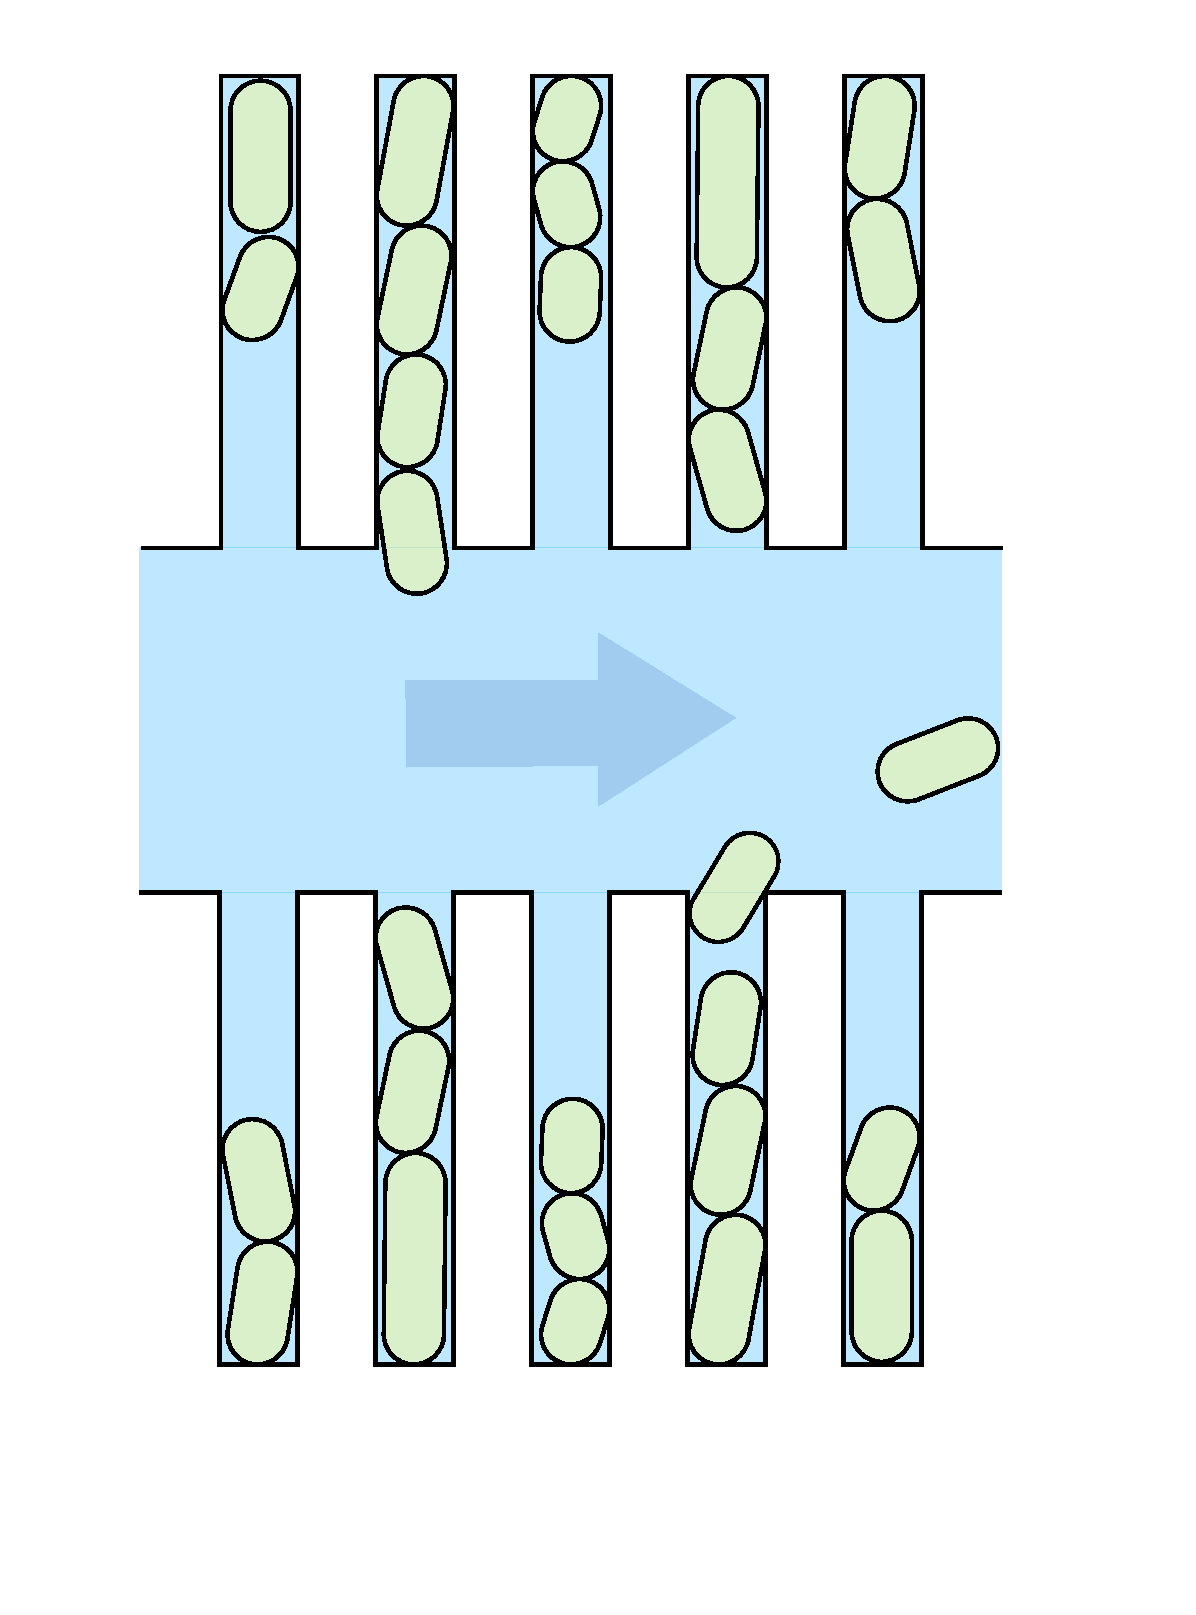
\includegraphics[width=55mm]{figure/MotherMachine_schematic_2D_cellLoaded.pdf}
    \caption{mother machine の構造。培地は主流路を矢印の向きに流れる。観察チャネルは主流路に垂直な行き止まりで、細胞が1列に入る。閉端の母細胞はとどまり、娘細胞は主流路へ押し出されて流される。}
    \label{fig:mm_schematic}
\end{figure}

\subsection{デバイスの構成}

本研究のデバイスは、Nakaoka と Wakamoto\cite{nakaoka2017aging} の設計に倣って自作した（図~\ref{fig:mm_layout}）。観察チャネルは幅 5.3 μm、高さ 6.2 μm、主流路（ドレイン）は幅 214 μm、高さ 19.75 μm である。\mynote{観察チャネルの長さと間隔、1視野に入る本数は設計ファイルで確認して書く}高さが2段階なので、鋳型は2層の SU-8 で作る。主流路の両端はチューブでシリンジと廃液容器につながり、シリンジポンプが培地を 2 mL/h で送る。細胞は観察チャネルの閉端側に入り、1列で増える。
\begin{figure}[H]
    \centering
    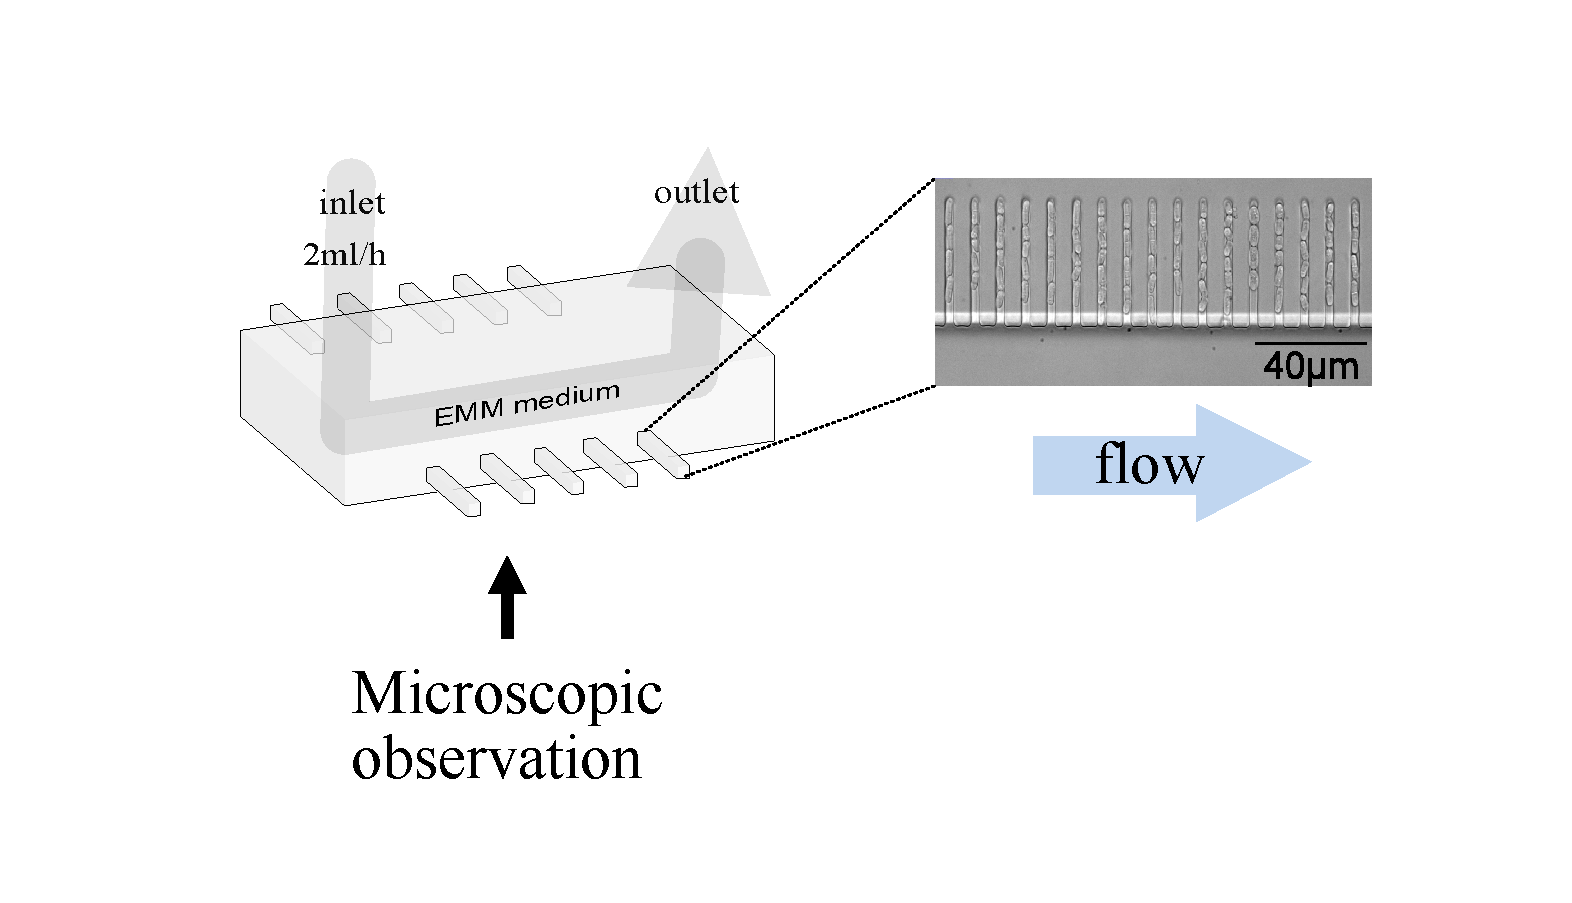
\includegraphics[width=0.9\linewidth]{figure/MotherMachine_channels_layout.pdf}
    \caption{デバイスの全体と観察チャネル。左: 入口からシリンジポンプで培地を送り、出口から廃液へ流す。観察はカバーガラス側から行う。右: 観察チャネルに分裂酵母が1列に入った明視野像。スケールバー 40 μm。}
    \label{fig:mm_layout}
\end{figure}

\subsection{作製}

作製の工程を図~\ref{fig:pdms_process}に示す。フォトマスクは、マスクブランクス（Clean Surface Technology）にマスクレス露光機（μMLA, Heidelberg Instruments）で描画した。観察チャネルとドレインは別のマスクにする。鋳型はシリコンウェハ（University Wafer）上の SU-8 を2層で作る。観察チャネル層は、SU-8 2 と SU-8 3005（MicroChem）の混合物を 3000 rpm で 30 s スピンコートし、65 °C で 1 min、95 °C で 2 min ソフトベークし、マスクアライナ（MA-20, Mikasa）でチャネルのマスクを通して 5 s の露光を3回行い、65 °C で 1 min、95 °C で 3 min の露光後ベークののち、SU-8 現像液（MicroChem）で現像してイソプロパノールで洗う。ドレイン層は、SU-8 3010（MicroChem）を 1500 rpm で 30 s スピンコートし、65 °C で 1 min、95 °C で 8 min ソフトベークし、1層目の合わせマークにドレインのマスクを合わせて 30 s 露光し、65 °C で 3 min、95 °C で 10 min の露光後ベークののち、同様に現像する。

PDMS は主剤と硬化剤（SYLGARD 184, Dow）を 10:1 で混ぜ、真空で 1 h 脱泡して鋳型に流し、65 °C で 12 h 以上硬化させる。切り出したブロックに直径 0.5 mm の生検トレパン（BP-A05F, Kai Medical）で入口と出口の穴を開け、エタノール中で超音波洗浄して 65 °C で乾かす。カバーガラス（Neo No.~1, Matsunami）は Contaminon LS-II の希釈液、超純水、エタノール、超純水の順に超音波洗浄し、0.1 M 水酸化ナトリウムで処理して超純水で洗い、140 °C で乾かす。PDMS ブロックとカバーガラスをプラズマ処理装置（FA-1, Samco）で 10 s 処理し、すぐに貼り合わせる。

日常の鋳造にはシリコンの鋳型を直接使わず、エポキシのレプリカを使う。鋳型から PDMS のネガ型を取り、それに2液性エポキシ（EA E-30CL, Loctite）を流して 24 h 以上硬化させる。このレプリカを型にして PDMS を鋳造する。作製の手順書（受け入れ条件とトラブル対応を含む）は Appendix C に置いた。
\begin{figure}[H]
    \centering
    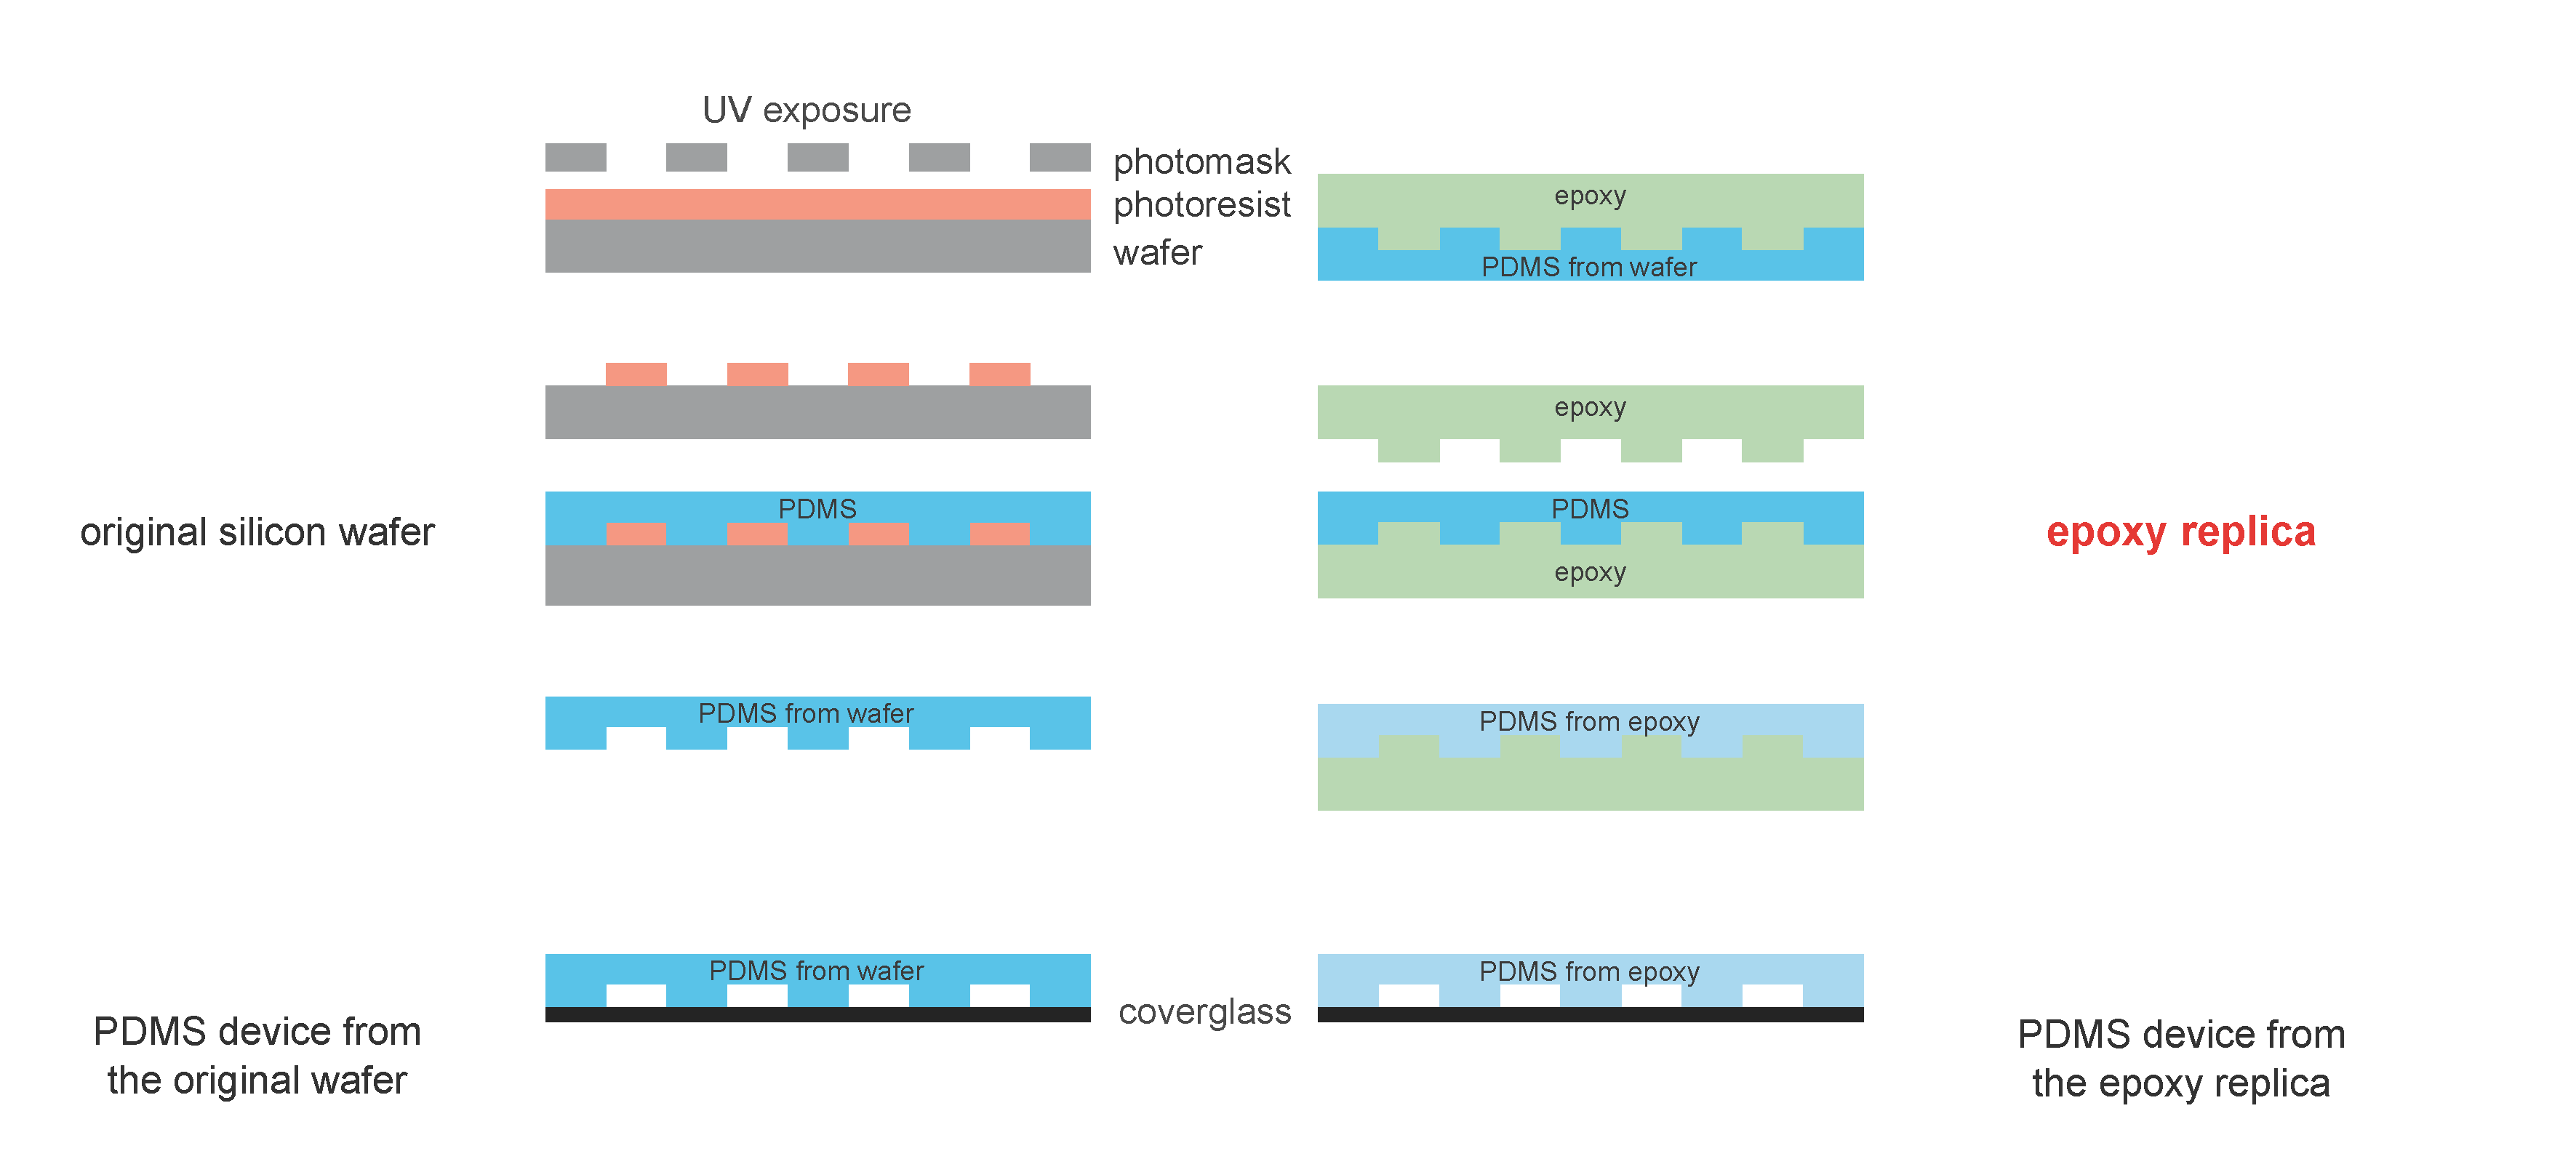
\includegraphics[width=0.95\linewidth]{figure/PDMS_fabrication_process.pdf}
    \caption{デバイスの作製工程。左: フォトマスクを通した露光で SU-8 の鋳型を作り、PDMS を鋳造してカバーガラスに接合する。右: 鋳型から取った PDMS のネガ型にエポキシを流してレプリカを作り、以後はレプリカから PDMS を鋳造する。}
    \label{fig:pdms_process}
\end{figure}

\section{細胞と長期タイムラプス計測}
\subsection{顕微鏡と環境}
Microscopy was conducted on an inverted Nikon Ti microscope (Nikon Instruments Inc.) fitted with a 40×/0.95 NA air objective. Samples were maintained at 30 °C with a stage-top incubator (Tokai Hit model ). The microscope hardware including motorized stage, shutters, Perfect Focus System (PFS) autofocus and image acquisition were controlled using Micro-Manager (v) open-source software.

\subsection{細胞株と培養条件}
% 性能評価に使った記録の株と培地。第3章 3.3.1 と同じなら1段落で再掲する。
% 実験1の株が HN0101（mNeonGreen）か FY18675（野生型）かは未確定。

\subsection{細胞の準備と導入}
Exponential-phase S. pombe cells cultured in EMM (2\% glucose) at 30°C were harvested from 20 mL cultures by centrifugation at 3,700 rpm for 5 min (HITACHI himac CT6E) to generate a 100-fold concentrated cell suspension. The concentrated suspension was loaded into the microfluidic device using a 1-mL syringe (Terumo).
To insert cells into the observation channels, the device was centrifuged at 1,200 rpm for 5 min, rotated 180°, and centrifuged again for 5 min. After confirming cell trapping within the observation channels by microscopy, EMM (2\% glucose) was perfused at 2 mL/h. Cells were allowed to settle until excess cells were completely flushed from the drain channels. Time-lapse imaging was then initiated after registering cell positions.

\subsection{培地交換と灌流}
For media exchanges to EMM (low\% glucose) or EMM (0\% glucose), the entire tubing system, including the connector, was replaced. The appearance of air bubbles in the connector, visualized by live microscopy, was used as the reference point to define the next frame as the time of media exchange.
Media perfusion was controlled by a syringe pump (Harvard ULTRA-P), maintaining a constant flow rate of 2 mL/h throughout the experiments to ensure stable environmental conditions.

\subsection{取得条件}
% 5分間隔・露光 60 ms・複数ステージ位置。論文 qpi-methods/sentence/20_methods.tex の Long-term time-lapse から日本語に起こす。

\subsection{参照グリッドの取得}
\label{sec:grid_acq}
% 細胞のそばに培地だけの領域が残らないので、計測前に stage 変位の 9×9 グリッド（0.1 µm 刻み）で参照像を撮る。
% 中心像を計測中のフィードバックの基準にする。論文 Reference acquisition から。

\subsection{タイムラプス計測と画像の取得}
% 蛍光顕微鏡（ORCA・LED・GFP-B）の記述で、QPI の計測系ではない。卒論の残りと思われる。
% Hsp104-GFP を第3章で使うなら 3.3 へ移す。使わないなら消す。
タイムラプス計測には,温度を正確に制御するためのサーモスタットチャンバー（TIZHB,TokaiHit）を備えた電動倒立顕微鏡（Nikon,Ti-E）を使用した.デジタルCMOSカメラ（ORCA C14440 ,浜松ホトニクス）,LED光源（Thorlabs）を組み合わせ,対物レンズはPlan Apo $\lambda$D 40x / 0.95(MRD70470,Nikon)を,GFP蛍光のフィルターキューブにはGFP-B(EX 460-500, DM 505, EM 510-560)を使用した.撮影はMicromanagerソフトウェア（https://micro-manager.org/）で制御し,5分間隔で画像を取得した.明視野画像の露光時間は50ミリ秒,GFP蛍光画像の露光時間は500ミリ秒とした.観察期間は実験条件によって異なり,192時間から240時間であった.長期間のタイムラプス撮影中には,焦点面の安定性を保つためにパーフェクト・フォーカス・システム（PFS）を使用した.すべての観察は30°Cで実施した.



\section{画像解析}
% 旧 Image analysis / Image Preprocessing / Volume estimation / Cell Segmentation の4節をここにまとめた。
% [from variational] 印の段落は別論文の手順の写し。論文 20_methods の対応する小節で置き換える。
To reduce post-processing time, each z-stack was cropped to a square region containing the cell(s) of interest and a border of at least 40 pixels, and the focal plane was identified. This cropping was accomplished first using FIJI v. 1.53c to identify regions of interest (ROIs) within a thresholded standard deviation z-projection image of each brightfield z-stack. Using custom Matlab R2019a (Mathworks) scripts, images were cropped to the ROIs and the standard deviation of the pixels in each ROI was computed. The focal plane was defined based on the image in the stack with the lowest standard deviation. Three images above and three images below the focal plane separated by 500 nm were used to quantify cytoplasmic density. Based on these images, the phase information was calculated using a custom Matlab script implementing a previously published algorithm (Bostan et al., 2016). In brief, this method relates the phase information of the cell to bright-field image intensity changes along the z-direction. Equidistant, out-of-focus images above and below the focal plane are used to estimate intensity changes at various defocus distances. A phase-shift map is reconstructed in a non-linear, iterative fashion to solve the transport-of-intensity equation.[from variational]

\subsection{位置合わせ}
% 各時点で ECC（並進のみ）で参照像に合わせる。下の段落は「空チャネルを引く」旧方式。論文はグリッド像を引く方式。今のコードがどちらかを QPI_Omni で確認。
To correct for sample drift during time-lapse imaging, we calculated alignment transformations using the Enhanced Correlation Coefficient (ECC) algorithm \cite{evangelidis2008parametric}. Alignment transformations were computed using images from empty channels (no cells present) to register against immobile channel structures. The resulting transformation matrices were stored and subsequently applied to cell-containing channel images using affine transformation. To isolate cellular phase signals from residual channel structures, the empty channel was subtracted from all subsequent frames, yielding differential phase images $\Delta\phi(x,y,t)$ representing only cellular refractive index contributions.

\subsection{背景差分}
\label{sec:bgsub}
% 各フレームの変位に最も近いグリッド像を背景として引く。残る 2π の倍数と線形成分は細胞のない領域で推定して除く。論文 Background subtraction から。
Using Matlab, images were background-corrected by fitting a Gaussian to the highest peak of the histogram (corresponding to the background pixels) of the phase-shift map and shifting every pixel so that the background intensity peak corresponded to zero phase shift. These background-corrected phase-shift maps were converted into binary images using watershedding for cell segmentation; where necessary, binary images were corrected manually to ensure accurate segmentation. Binary images were segmented using Morphometrics (Ursell et al., 2017) to generate subpixel-resolved cell outlines.

\subsection{培地屈折率の校正}
% BSA 濃度系列（0–5% w/v）の灌流。論文 Calibration から。下の段落の BSA 100 mg/mL 1点は別論文の写し。
To convert the mean intensity of the phase-shift within each cell into absolute concentration (in units of mg/mL), the mean of all cells across all time points was first calculated. Then, the decrease in phase shift induced by a prescribed concentration of BSA (typically 100 mg/mL) was defined as the difference between the mean of the phase shifts before and after the BSA imaging time point and the phase shift during the BSA time point. This difference in intensity established the calibration scaling between phase shift intensity and the concentration of BSA (Figure 1B). The cytoplasmic density of each cell was then calculated by dividing the mean phase shift of the cell by the aforementioned scaling factor. The mass of each cell was inferred from its mean density and volume.[from variational]

\subsection{セグメンテーション}
明視野（BF）画像のセグメンテーションは,顕微鏡における細胞セグメンテーションに一般的に使用される深層学習ベースのアルゴリズムであるOmnipose\cite{cutler2022omnipose}の半自動ワークフローを用いてセグメンテーションした.Omnipose は,大規模なパラメータチューニングをすることなく,様々なタイプの画像を正確にセグメントできることで知られている.BF画像のセグメンテーションを容易にするために,Omniposeモデルは,パラメータ調整なしで,GFP蛍光画像から得られたマスク画像からなるグランドトゥルースデータを用いて学習された.得られた学習済みモデルをBF画像に適用した(図4). 
\begin{figure}[htbp]
\centering
\includegraphics[width=50mm]{example-image}
\caption{\textnormal{\textbf{Omniposeインターフェース}Omniposeではリアルタイムのフィードバックデータのインタラクティブな解析を可能にする.表示されている生データはBF画像に訓練済みのモデルを用いて,セグメンテーションを行ったマスクを重ね合わせた図}}
\end{figure}

Cell boundaries were detected using Omnipose \cite{cutler2022omnipose}, a deep learning-based segmentation method optimized for bacterial morphology. We trained a custom Omnipose model on approximately 3000 manually annotated S. pombe cells. Training images were first manually annotated using the Omnipose GUI to generate ground truth segmentation masks. Segmentation masks were converted to binary outlines by detecting pixel discontinuities at cell boundaries using morphological operations. Specifically, boundaries were identified where mask values differed from their four-connected neighbors, generating single-pixel-width contours.


\subsection{系譜追跡}
% 面積でフレーム間を連結する。論文 lineage tracking から。

\subsection{細胞の形状と体積}
% 楕円 Fourier 記述子で輪郭を平滑化し、medial axis に垂直な幅から回転対称で体積。論文 Cell geometry から。
戸田さんの哺乳類細胞の体積推定や他のrod shape近似の書き方を調べる

Each cell outline was skeletonized using custom Matlab code as follows. First, the closest-fitting rectangle around each cell was used to define the long axis of the cell. Perpendicular to the long axis, sectioning lines at 250 nm intervals and their intersection with the cell contour were computed. The centerline was then updated to run through the midpoint of each sectioning line between the two contour-intersection points. The slope of each sectioning line was updated to be perpendicular to the slope of the centerline around the midpoint. Sectioning lines that crossed a neighboring line were removed. Cell volume and surface area were calculated by summing the volume or area of each section, assuming rotational symmetry. Volume and area of the poles were calculated assuming a regular spherical cap.

\subsection{乾燥質量}
% Barer (1952)、屈折率増分 0.18 mL/g、位相の面積分から乾燥質量濃度。論文 Dry mass から。2.1 の 0.19 と揃える。

\section{性能評価}
\label{sec:performance}
% Figure 2（校正・精度）と Figure 3（位相ノイズ・グリッド・ドリフト・既知シフトの回収）はここ。
% これらは手法の検証図なので、実験1のデータを待たずに書ける。

\subsection{位相感度の理論}
% 旧「Phase sensitivity」節をここへ移した。式は 2.9 でしか使わない。

To discuss the OPD precision of off-axis DH, determined by the temporal OPD noise, we first add the noise term $z_{m,n}^{\mathrm{DH}}$ to \eqref{eq:hologram_DH}, such that
\begin{equation}
I_{m,n}^{'\mathrm{DH}} = J_{m,n}^{\mathrm{non-int}} + J_{m,n}^{\mathrm{int}} e^{-i(k_m^{\mathrm{off-axis}}m + k_n^{\mathrm{off-axis}}n)} + (J_{m,n}^{\mathrm{int}})^* e^{i(k_m^{\mathrm{off-axis}}m + k_n^{\mathrm{off-axis}}n)} + z_{m,n}^{\mathrm{DH}}.
\end{equation}
The OPD image containing noise is represented by
\begin{align}
\phi'_{m,n} &= \arg\left[\mathrm{LP}\left(\frac{I_{m,n}^{'\mathrm{DH}} e^{i(k_m^{\mathrm{off-axis}}m + k_n^{\mathrm{off-axis}}n)}}{|J_{m,n}^{\mathrm{int}}|}\right)\right] \nonumber \\
&= \arg\left[e^{i\phi_{m,n}}\left(1 + \frac{\mathrm{LP}(z_{m,n}^{\mathrm{DH}} e^{i(k_m^{\mathrm{off-axis}}m + k_n^{\mathrm{off-axis}}n)})}{|J_{m,n}^{\mathrm{int}}| e^{i\phi_{m,n}}}\right)\right] \nonumber \\
&= \phi_{m,n} + \frac{z_{m,n}^{\mathrm{DH}} \sin(k_m^{\mathrm{off-axis}}m + k_n^{\mathrm{off-axis}}n - \phi_{m,n}) \ast H_{m,n}}{|J_{m,n}^{\mathrm{int}}|},
\end{align}
where $H_{m,n}$ denotes the IFT of the pupil function $h_{k,l}$ for LP filtering, and $\ast$ represents convolution. The temporal OPD standard deviation at each spatial pixel $\sigma_{\phi'}^{\mathrm{DH}}$ can be obtained by calculating the square root of the variance of $\phi'_{m,n}$ as
\begin{align}
\sigma_{\phi'}^{\mathrm{DH}} &= \sqrt{\mathrm{Var}(\phi'_{m,n})} = \frac{1}{|J_{m,n}^{\mathrm{int}}|} \sqrt{[\mathrm{Var}(z_{m,n}^{\mathrm{DH}}) \sin^2(k_m^{\mathrm{off-axis}}m + k_n^{\mathrm{off-axis}}n - \phi_{m,n})] \ast H_{m,n}^2} \nonumber \\
&= \frac{1}{|J_{m,n}^{\mathrm{int}}|} \sqrt{\left[\mathrm{Var}(z_{m,n}^{\mathrm{DH}}) \frac{1 - \cos 2(k_m^{\mathrm{off-axis}}m + k_n^{\mathrm{off-axis}}n - \phi_{m,n})}{2}\right] \ast H_{m,n}^2}. \label{eq:sigma_phi_DH}
\end{align}

In the case of optical shot-noise-limited detection, $\mathrm{Var}(z_{m,n}^{\mathrm{DH,shot}})$ is given by
\begin{equation}
\label{eq:var_shot}
\mathrm{Var}(z_{m,n}^{\mathrm{DH,shot}}) = \mathrm{Mean}(I_{m,n}^{\mathrm{DH}}) = J_{m,n}^{\mathrm{non-int}} + 2|J_{m,n}^{\mathrm{int}}| \cos(\phi_{m,n} - k_m^{\mathrm{off-axis}}m - k_n^{\mathrm{off-axis}}n).
\end{equation}
All terms outside the LP bandwidth, such as $\cos 2(k_m^{\mathrm{off-axis}}m + k_n^{\mathrm{off-axis}}n - \phi_{m,n})$ in \eqref{eq:sigma_phi_DH} and $\cos(\phi_{m,n} - k_m^{\mathrm{off-axis}}m - k_n^{\mathrm{off-axis}}n)$ in \eqref{eq:var_shot}, are removed by the LP-filtering operation $\ast H_{m,n}$. Because $h_{k,l}$ is unity within its passband and zero elsewhere, $H_{m,n}^2$ can be approximated by the delta function $\delta_{m,n}$, and the summation of its amplitude over the entire pixel range is expressed as
\begin{equation}
\label{eq:H_sum}
\sum_{m,n} H_{m,n}^2 = \sum_{k,l} h_{k,l}^2 \cdot \frac{A_{\mathrm{aperture}}}{A_{\mathrm{sensor}}},
\end{equation}
where $A_{\mathrm{sensor}}$ is the total number of sensor pixels and $A_{\mathrm{aperture}}$ is the number of pixels inside the LP bandwidth. By substituting \eqref{eq:H_sum} into \eqref{eq:sigma_phi_DH}, we obtain the optical shot-noise-limited OPD precision as
\begin{equation}
\label{eq:sigma_shot}
\sigma_{\phi'}^{\mathrm{DH,shot}} = \frac{\sqrt{|J_{m,n}^{\mathrm{non-int}}| \ast H_{m,n}^2}}{\sqrt{2}|J_{m,n}^{\mathrm{int}}|} = \sqrt{\frac{|J_{m,n}^{\mathrm{non-int}}|}{2|J_{m,n}^{\mathrm{int}}|^2}} \sqrt{\frac{A_{\mathrm{aperture}}}{A_{\mathrm{sensor}}}}.
\end{equation}

Equation~\eqref{eq:sigma_shot} can be extended to obtain the OPD precision including both the optical shot noise and the sensor's read-out noise as
\begin{equation}
\sigma_{\phi'}^{\mathrm{DH,shot+sensor}} = \sqrt{\frac{|J_{m,n}^{\mathrm{non-int}}| + \mathrm{Var}(z_{m,n}^{\mathrm{sensor}})}{2|J_{m,n}^{\mathrm{int}}|^2}} \sqrt{\frac{A_{\mathrm{aperture}}}{A_{\mathrm{sensor}}}},
\end{equation}
where $\mathrm{Var}(z_{m,n}^{\mathrm{sensor}})$ is the variance of the sensor read-out noise.

Using the visibility $V = 2|J_{m,n}^{\mathrm{int}}|/J_{m,n}^{\mathrm{non-int}}$ and noting that $J_{m,n}^{\mathrm{non-int}} = |U_{s,m,n}|^2 + |U_{r,m,n}|^2$ is the mean intensity (in units of electrons), the shot-noise-limited phase sensitivity can be written as
\begin{equation}
\sigma_{\phi}^{\mathrm{shot}} = \frac{1}{V} \sqrt{\frac{2}{J_{m,n}^{\mathrm{non-int}}}} \sqrt{\frac{A_{\mathrm{aperture}}}{A_{\mathrm{sensor}}}} = \frac{1}{V\sqrt{N_e}} \sqrt{\frac{2A_{\mathrm{aperture}}}{A_{\mathrm{sensor}}}},
\end{equation}
where $N_e = J_{m,n}^{\mathrm{non-int}}$ is the total number of electrons.

In common-path off-axis holography with background subtraction, the noise propagates from both sample and background measurements. Since the measurements are independent, the variance becomes $\mathrm{Var}[\Delta I] = 2\sigma_I^2$, yielding
\begin{equation}
\sigma_{\phi}^{\mathrm{bg\ sub}} = \sqrt{2} \times \sigma_{\phi}^{\mathrm{shot}} = \frac{\sqrt{2}}{V\sqrt{N_e}} \sqrt{\frac{2A_{\mathrm{aperture}}}{A_{\mathrm{sensor}}}} = \frac{2}{V\sqrt{N_e}} \sqrt{\frac{A_{\mathrm{aperture}}}{A_{\mathrm{sensor}}}}.
\end{equation}

The phase sensitivity exhibits a quadratic dependence on visibility ($\sigma_{\phi} \propto V^{-1}$) and a square-root dependence on the number of electrons ($\sigma_{\phi} \propto N_e^{-1/2}$), making visibility optimization critical for achieving high sensitivity.


\subsection{位相ノイズ}
% 連続フレーム差の空間標準偏差/√2 を細胞のない領域で測り、上の shot-noise 限界と比べる。Figure 3A（測り直し要）。

\subsection{参照グリッド登録の精度}
% 公称ステージ変位と実測変位の差、誤差ベクトル。Figure 3B（対応表を 32 bit 実数で作り直してから）。

\subsection{ドリフト}
% 記録全長での位置ずれ、補正あり／なし。Figure 3C（確定済み）。

\subsection{既知シフトの回収}
% 細胞のない領域に既知の sub-pixel 並進を与えて回収、MAE 3.8 nm。Figure 3D（確定済み）。

\subsection{濃度校正の直線性}
% BSA 系列に対する位相の線形。Figure 2（ver2 未決）。

\section{考察}
% 他の QPI 系・他の密度計測法との比較と、この系の限界。論文 qpi-methods/sentence/40_discussion.tex から。

\section{まとめ}
% 何を、どの精度で、どれだけ長く測れるか（数値は 2.9 から）。第3章で何に使うか1文。
